\section{Volumes of Revolution}
As we did for areas between curves, we can use our knowledge of
integrals to compute the volume of certain objects: ones obtained
by rotating a region about a horizontal or vertical line!

\begin{Remark}{}{}
    For more general shapes, we need multivariable methods. These are
    explored in MATH 237!
\end{Remark}

Let's get a formula!

\underline{Areas}:
\begin{itemize}
    \item Area of one infinitesimally thin rectangle: $ f(x)\odif{x} $
    \item Overall area: $ \displaystyle \int_{a}^{b} f(x)\odif{x}  $
\end{itemize}
\underline{Volumes} (rotate $ f $ around $ x $-axis):
\begin{itemize}
    \item Volume of one infinitesimally thin slice: $ A(x)\odif{x} $
    \item Overall volume: $ \displaystyle \int_{a}^{b} A(x)\odif{x} $
\end{itemize}

So, we just need to determine $ A(x) $ in each case! There are
a few different methods we will use.

The two main methods are:
\begin{enumerate}[label=(\Roman*)]
    \item Washers/disks (i.e., cross-sections)
    \item Cylindrical shells
\end{enumerate}

\subsection*{Method 1: Washers/disks}

First, let's recall the area formulas:

\begin{figure}
    \centering
    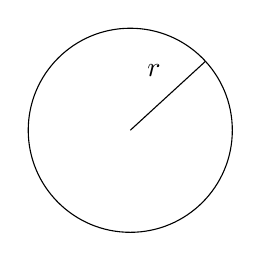
\begin{tikzpicture}[x=0.75pt,y=0.75pt,yscale=-1,xscale=1]
        %uncomment if require: \path (0,123); %set diagram left start at 0, and has height of 123

        %Shape: Circle [id:dp2971916951811683] 
        \draw   (31,59.83) .. controls (31,32.68) and (53.01,10.67) .. (80.17,10.67) .. controls (107.32,10.67) and (129.33,32.68) .. (129.33,59.83) .. controls (129.33,86.99) and (107.32,109) .. (80.17,109) .. controls (53.01,109) and (31,86.99) .. (31,59.83) -- cycle ;
        %Straight Lines [id:da8239626600891564] 
        \draw    (80.17,59.83) -- (116.33,26.67) ;

        % Text Node
        \draw (87.17,26.9) node [anchor=north west][inner sep=0.75pt]    {$r$};
    \end{tikzpicture}
    \caption{Area of a disk with radius $ r $: $ \pi r^2 $}
\end{figure}

\begin{figure}
    \centering
    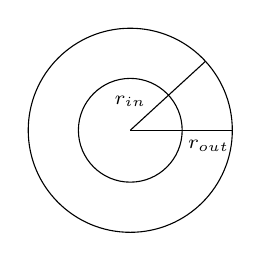
\begin{tikzpicture}[x=0.75pt,y=0.75pt,yscale=-1,xscale=1]
        %uncomment if require: \path (0,123); %set diagram left start at 0, and has height of 123

        %Shape: Circle [id:dp2971916951811683] 
        \draw   (31,59.83) .. controls (31,32.68) and (53.01,10.67) .. (80.17,10.67) .. controls (107.32,10.67) and (129.33,32.68) .. (129.33,59.83) .. controls (129.33,86.99) and (107.32,109) .. (80.17,109) .. controls (53.01,109) and (31,86.99) .. (31,59.83) -- cycle ;
        %Straight Lines [id:da8239626600891564] 
        \draw    (80.17,59.83) -- (116.33,26.67) ;
        %Shape: Circle [id:dp7459673192558707] 
        \draw   (55.17,59.83) .. controls (55.17,46.03) and (66.36,34.83) .. (80.17,34.83) .. controls (93.97,34.83) and (105.17,46.03) .. (105.17,59.83) .. controls (105.17,73.64) and (93.97,84.83) .. (80.17,84.83) .. controls (66.36,84.83) and (55.17,73.64) .. (55.17,59.83) -- cycle ;
        %Straight Lines [id:da52555392875757] 
        \draw    (129.33,59.83) -- (80.17,59.83) ;

        % Text Node
        \draw (106.75,63.23) node [anchor=north west][inner sep=0.75pt]  [font=\scriptsize]  {$r_{\text{out}}$};
        % Text Node
        \draw (80.17,42) node [anchor=north] [inner sep=0.75pt]  [font=\scriptsize]  {$r_{\text{in}}$};


    \end{tikzpicture}
    \caption{Area of a washer with outer radius $ r_{\text{out}} $ and inner radius $ r_\text{in} $:
        $ \pi(r_{\text{out}})^2-\pi(r_\text{in})^2 $}
\end{figure}


\begin{Example}{}{}
    Find the volume of the solid obtained by rotating $ f(x)=\sqrt{x-1} $ about the $ x $-axis
    from $ x=1 $ to $ x=5 $.

    \begin{center}
        \begin{tikzpicture}
            \begin{axis}[ylabel = $y$, xlabel = $x$, x post scale=1.4]
                \filldraw[red!20] (5,0) circle [x radius=0.25, y radius=2];
                \filldraw[red!20] (2.5,0) circle [x radius=0.25, y radius=1.2];
                \addplot[blue, domain=1:6, name path=F] {sqrt(x-1)} node [pos = 0.5, above left] {$y=\sqrt{x-1}$};
                \addplot[blue, domain=1:6] {-sqrt(x-1)};
                \addplot[black, domain=0:6] {0} node [pos = 0.1, below] {\tiny{$x$-axis ($y=0$)}};
                \draw[-] (0,-2) -- (0,2) node[above] {$x=0$};
                \draw[-] (5,-2) -- (5,2) node[above] {$x=5$};
                \node at (2.5,0.5) {\scriptsize $A(x)$};
            \end{axis}
        \end{tikzpicture}
    \end{center}

    \textbf{Solution.} The cross-section is a disk with radius $ \sqrt{x-1} $. So
    \[ A(x)=\pi( \sqrt{x-1} )^2=\pi(x-1) \]
    and
    \begin{align*}
        \text{Volume}
         & =\int_{1}^{5} A(x)\odif{x}                        \\
         & =\int_{1}^{5} \pi(x-1)\odif{x}                    \\
         & =\pi\left[ \frac{x^2}{2} -x \right]_1^5           \\
         & =\pi\left( \frac{25}{2} -5-\frac{1}{2} +1 \right) \\
         & =8\pi
    \end{align*}
\end{Example}

Note that you don't need to draw the full 3-D image, just one area slice is enough!

\begin{Example}{}{}
    Rotate the area between $ y=\sqrt{x} $ and $ y=x^2 $ about the line $ y=1 $.

    \begin{center}
        \begin{tikzpicture}
            \begin{axis}[ylabel = $y$, xlabel = $x$]
                \filldraw[red!20] (0.3,1) circle [x radius=0.2, y radius=0.9];
                \filldraw[white] (0.3,1) circle [x radius=0.1, y radius=0.45];
                \addplot[blue, domain=0:1.25, name path=F] {sqrt(\x)} node [pos = 1, right] {$y=\sqrt{x}$};
                \addplot[red, domain=0:1.25, name path=G] {x^2} node [pos = 1, below right] {$y=x^2$};
                \addplot[black, domain=0:1.5] {1};
                \draw[Purple, very thick] (0.3,0.3^2) -- (0.3,1);
                \draw[ForestGreen, very thick] (0.28,0.5477) -- (0.28,1);
            \end{axis}
        \end{tikzpicture}
    \end{center}

    \textbf{Solution.} The cross-section is a washer with $ \textcolor{Purple}{r_{\text{out}}=1-x^2} $ and
    $ \textcolor{ForestGreen}{r_{\text{in}}=1-\sqrt{x}} $. So,
    \begin{align*}
        A(x)
         & =\pi(r_{\text{out}})^2-\pi(r_\text{in})^2   \\
         & =\pi\left[ (1-x^2)^2-(1-\sqrt{x})^2 \right] \\
         & =\pi(1-2x^2+x^4-1+2\sqrt{x}-x)              \\
         & =\pi(x^4-2x^2+2\sqrt{x}-x)
    \end{align*}
    and
    \begin{align*}
        \text{Volume}
         & =\int_{0}^{1} A(x)\odif{x}                                                                       \\
         & =\pi \int_{0}^{1} x^4-2x^2+2x^{\sfrac{1}{2}}-x\odif{x}                                           \\
         & =\pi\left[ \frac{x^5}{5} -\frac{2}{3} x^3+\frac{4}{3} x^{\sfrac{3}{2}}-\frac{x^2}{2} \right]_0^1 \\
         & =\pi\left( \frac{1}{5} -\frac{2}{3} +\frac{4}{3} -\frac{1}{2} \right)                            \\
         & =\frac{11\pi}{30}
    \end{align*}
\end{Example}


\begin{Example}{}{}
    Rotate the region between $ x=y^2 $ and $ x=2y $ about the $ y $-axis.

    \begin{center}
        \includegraphics[width=0.6\textwidth]{diagram 4.pdf}
    \end{center}

    \textbf{Solution.} First, points of intersection: $ y^2=2y\implies y=0,2 $.
    The cross-section is a washer with $ \color[rgb]{0.5,0,0.5} r_{\text{out}}=2y $ and
    $ \color[rgb]{0,0.5,0}  r_{\text{in}}=y^2 $. So,
    \begin{align*}
        A(y)
         & =\pi\left(2y\right)^2-\pi\left(y^2\right)^2 \\
         & =\pi\left( 4y^2-y^4 \right)
    \end{align*}
    and
    \begin{align*}
        \text{Volume}
         & =\pi \int_{0}^{2} 4y^2-y^4\odif{y} \\
         & =\text{exercise}                   \\
         & =\frac{64\pi}{15}
    \end{align*}
\end{Example}

We can see that washers/disks arise when we rotate functions of $ x $ about
a horizontal line or functions of $ y $ about a vertical line.

We can't use it all the time though, for example: rotate the region below
$ y=2x^2-x^3 $ about the $ y $-axis from $ x=0 $ to $ x=2 $.

\begin{center}
    \includegraphics[width=0.6\textwidth]{diagram 5.pdf}
\end{center}

We need another method!

\subsection*{Method 2: Cylindrical shells}

Instead of using cross-sections, we can use cylindrical shells (think soup can labels)
to divide the volume up!

Q\@: What is the area of a cylindrical shell with base radius $ r $ and height $ h $?

\begin{center}
    \includegraphics[width=0.6\textwidth]{diagram 6.pdf}
\end{center}

So area is $ 2\pi rh $. So, we only need to determine $ r $ and $ h $!

Back to the difficult example:
\begin{Example}{}{}
    Rotate the region below $ y=2x^2-x^3 $ about the $ y $-axis from $ x=0 $ to $ x=2 $. Find the volume.
    \begin{center}
        \begin{tikzpicture}
            \begin{axis}[ylabel = $y$, xlabel = $x$]
                \addplot[blue, domain=-0.5:2.25, name path=F] {2*x^2-x^3} node [pos = 0.45, above right] {$y=2x^2-x^3$};
                \addplot[blue, domain=-0.5:2.25, name path=G] {0} node [pos = 0.5, below] {$y=0$};
                \addplot[fill=red!10] fill between [of=F and G, soft clip={domain=0:2}];
                \draw[-] (0,1) -- (0,-0.75) node[below] {$x=0$};
                \draw[-] (2,1) -- (2,-0.75) node[below left] {$x=2$};
                \draw[ForestGreen, very thick] (0,0.703125) -- (0.75,0.703125);
                \draw[Purple, very thick] (0.75,0) -- (0.75,0.703125);
            \end{axis}
        \end{tikzpicture}
    \end{center}
    \textbf{Solution.}
    \begin{itemize}
        \item Intersection points: $ 2x^2-x^3=0\implies x=0,2 $.
        \item \textcolor{ForestGreen}{$ r=x $}.
        \item \textcolor{Purple}{$ h=2x^2-x^3-0=2x^2-x^3 $}.
    \end{itemize}
    Hence, the area is $ A(x)=2\pi x(2x^2-x^3) $. Therefore, the volume is
    \[ V=\int_{0}^{2}2\pi x(2x^2-x^3)\odif{x}=\frac{16\pi}{5}. \]
\end{Example}

\begin{Example}{}{}
    Find the volume in each case.
    \begin{enumerate}[label=(\roman*)]
        \item Rotate the region between $ y=x^2 $ and $ y=6x-x^2 $
              about the $ y $-axis.
              \begin{center}
                  \begin{tikzpicture}
                      \begin{axis}[ylabel = $y$, xlabel = $x$]
                          \addplot[blue, domain=-0.5:3, name path=F] {x^2} node [pos = 0.5, below right] {$y=x^2$};
                          \addplot[red, domain=-0.5:3, name path=G] {6*x - x^2} node [pos = 0.8, above left] {$y=6x-x^2$};
                          \addplot[fill=red!10] fill between [of=F and G, soft clip={domain=0:3}];
                          \draw[-] (0,10) -- (0,-2) node[below] {$x=0$};
                          \draw[Purple, very thick] (1,1) -- (1,5);
                          \draw[ForestGreen, very thick] (1,1) -- (0,1);
                      \end{axis}
                  \end{tikzpicture}
              \end{center}
              \textbf{Solution.}
              \begin{itemize}
                  \item Intersection points: $ x^2=6x-2x^2\implies x=0,2 $.
                  \item \textcolor{ForestGreen}{$ r=x $}.
                  \item \textcolor{Purple}{$ h=6x-2x^2-x^2=6x-3x^2 $}.
              \end{itemize}
              Hence, the area is $ A(x)=2\pi x(6x-3x^2) $. Therefore, the volume is
              \[ V
                  =\int_{0}^{2} 2\pi x(6x-3x^2)\odif{x} \\
                  =8\pi.  \]
        \item Rotate the region bounded by $ y=4x-x^3 $ and $ y=3 $ about
              $ x=1 $.
              \begin{center}
                  \begin{tikzpicture}
                      \begin{axis}[ylabel = $y$, xlabel = $x$]
                          \addplot[blue, domain=0.5:4, name path=F] {3} node [pos = 1, below] {$y=3$};
                          \addplot[red, domain=0.5:4, name path=G] {4*x - x^2} node [pos = 0.8, below left] {$y=4x-x^3$};
                          \addplot[fill=red!10] fill between [of=F and G, soft clip={domain=1:3}];
                          \draw[-] (1,0) -- (1,3.75) node[above] {$x=1$};
                          \draw[Purple, very thick] (1.5,3) -- (1.5,3.75);
                          \draw[ForestGreen, very thick] (1,3) -- (1.5,3);
                      \end{axis}
                  \end{tikzpicture}
              \end{center}
              \textbf{Solution.}
              \begin{itemize}
                  \item Intersection points: $ 4x-x^2=3\implies x=1,3 $.
                  \item \textcolor{ForestGreen}{$ r=x-1 $}.
                  \item \textcolor{Purple}{$ h=4x-x^3-3 $}.
              \end{itemize}
              Hence, the area is $ A(x)=2\pi(x-1)(4x-x^2-3) $. Therefore, the volume is
              \[ V
                  =\int_{1}^{3}2\pi(x-1)(4x-x^2-3)\odif{x}
                  =\frac{8\pi}{3}. \]
    \end{enumerate}
\end{Example}

We will now look at some more practice examples, but first a handy table:

\begin{table}[!htbp]
    \centering
    \begin{tabular}{ccc}
        What are you rotating the function around? & Functions of $ x $ & Functions of $ y $ \\
        \midrule
        Vertical line                              & Cylindrical shells & Washers/disks      \\
        Horizontal line                            & Washers/disks      & Cylindrical shells
    \end{tabular}
\end{table}

\begin{Example}{More Practice}{}
    Set up, but don't evaluate the integral(s) that would give
    the desired volume.

    \begin{enumerate}[label=(\roman*)]
        \item Rotate the region bounded by $ xy=1 $, $ x=0 $, $ y=1 $, $ y=3 $,
              around the $ x $-axis.

              \begin{center}
                  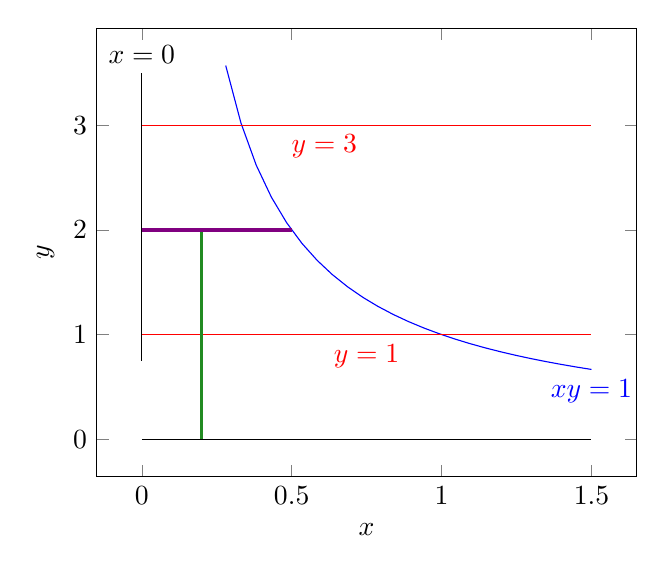
\begin{tikzpicture}
                      \begin{axis}[ylabel = $y$, xlabel = $x$]
                          \addplot[blue, domain=0.28:1.5] {1/x} node [pos = 1, below] {$xy=1$};
                          \addplot[red, domain=0:1.5] {1} node [pos = 0.5, below] {$y=1$};
                          \addplot[red, domain=0:1.5] {3} node [pos = 0.5, below left] {$y=3$};
                          \addplot[black, domain=0:1.5] {0};
                          \draw[-] (0,0.75) -- (0,3.5) node[above] {$x=0$};
                          \draw[ForestGreen, very thick] (0.2,0) -- (0.2,2);
                          \draw[Purple, very thick] (0,2) -- (0.5,2);
                      \end{axis}
                  \end{tikzpicture}
              \end{center}

              \textbf{Solution 1.} Cylindrical shell:
              \begin{itemize}
                  \item Intersection points: $ x=1,3 $.
                  \item \textcolor{ForestGreen}{$ r=y $}.
                  \item \textcolor{Purple}{$ h=1/y $}.
              \end{itemize}
              Hence, the area is $ A(x)=2\pi y(1/y)=2\pi $. Therefore, the volume is
              \[ V=\int_{1}^{3} 2\pi\odif{y}=4\pi. \]
              \textbf{Solution 2.} For fun, can we do it using washers/disks?

              A\@: Yes! Just work with $ x $ and not $ y $.
              \begin{itemize}
                  \item $ \displaystyle  r_{\text{out}}=\begin{cases}
                                3   & 0\leqslant x\leqslant 1/3   \\
                                1/x & 1/3 \leqslant x \leqslant 1
                            \end{cases} $
                  \item $ r_{\text{in}}=1 $,
              \end{itemize}
              Therefore, the volume is
              \[ V=\pi\int_{0}^{1/3} 3^2-1^2\odif{x}
                  +\pi\int_{1/3}^{1} 1/x^2-1^2\odif{x}=4\pi. \]
              This method was more difficult, because $ r_{\text{out}} $ changes, but it is still valid!

        \item Region bounded by $ x=(y-1)^2 $, $ x=y+1 $, about $ x=-1 $.
              \begin{center}
                  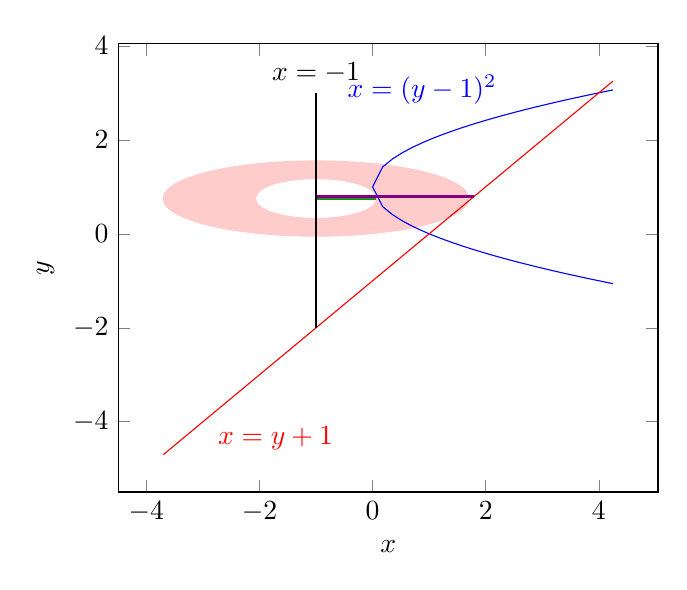
\begin{tikzpicture}
                      \begin{axis}[ylabel = $y$, xlabel = $x$]
                          \filldraw[red!20] (-1,0.75) circle [x radius=2.7, y radius=0.8];
                          \filldraw[white] (-1,0.75) circle [x radius=1.05, y radius=0.4];
                          \addplot[blue, domain=0:4.25] {sqrt(\x)+1} node [pos = 0.6, above left] {$x=(y-1)^2$};
                          \addplot[blue, domain=0:4.25] {-sqrt(\x)+1};
                          \addplot[red, domain=-3.7:4.25] {x-1} node [pos = 0.1, below right] {$x=y+1$};
                          \addplot[ForestGreen, domain=-1:0.0625, very thick] {0.75}; % inner green
                          \addplot[Purple, domain=-1:1.8, very thick] {0.8}; % outer purple
                          \draw[-] (-1,-2) -- (-1,3) node[above] {$x=-1$};
                      \end{axis}
                  \end{tikzpicture}
              \end{center}
              \textbf{Solution.}
              \begin{itemize}
                  \item Intersection points $ (y-1)^2=y+1\implies y=0,3 $.
                  \item \textcolor{Purple}{$ r_{\text{out}}=y+1-(-1)=y+2 $}.
                  \item \textcolor{ForestGreen}{$ r_{\text{in}}=(y-1)^2-(-1)=(y-1)^2+1 $}.
              \end{itemize}
              Therefore, the volume is
              \[ V=\pi \int_{0}^{3} (y+2)^2-\bigl[ (y-1)^2+1 \bigr]^2\odif{y}. \]
    \end{enumerate}
\end{Example}

\chapter{Differential Equations}
\section{Introduction to Differential Equations}
\begin{Definition}{Ordinary Differential Equation}{}
    An equation containing derivatives of a dependent variable (i.e., function) $ y=f(x) $
    is called an \textbf{ordinary differential equation} (ODE).
\end{Definition}

\begin{Remark}{}{}
    To contrast, there are also partial differential equations for multivariable functions.
\end{Remark}

\begin{Example}{Ordinary Differential Equations}{}
    \begin{itemize}
        \item $ y^\prime+2y=e^x $
        \item $ y^{\prime\prime}+y^\prime+y=0 $
        \item $ x^2y^\prime+y=31 $
    \end{itemize}
\end{Example}

\begin{Definition}{Order}{}
    The \textbf{order} of an ODE is the order of the highest derivative that appears.
\end{Definition}

\begin{Example}{Order}{}
    \begin{itemize}
        \item $ y^{\prime\prime}+y^3=0 $: order 2
        \item $ x^2\odv[order=2]{y}{x} +\odv{y}{x} =y $: order 2
        \item $ y^\prime+y=\sin(x) $: order 1
    \end{itemize}
\end{Example}

\begin{Definition}{Linear}{}
    An ODE is called \textbf{linear} if it contains only linear functions in $ y $, $ y^\prime $,
    $ y^{\prime\prime} $, etc.
\end{Definition}

\begin{Example}{Linear and Non-linear ODEs}{}
    \begin{itemize}
        \item $ 3y^{\prime\prime}+2x^3y=\cos(x) $: linear
        \item $ y^2+y^\prime=0 $: not linear $ (y^2) $
        \item $ yy^\prime=0 $: not linear
    \end{itemize}
\end{Example}

\begin{Definition}{General Solution}{}
    The \textbf{general solution} of an ODE is the collection of all possible
    solutions including arbitrary constants.
\end{Definition}

\begin{Definition}{Particular Solution}{}
    A \textbf{particular solution} is a solution in which all arbitrary constants
    have been determined.
\end{Definition}

\begin{Definition}{Initial Conditions}{}
    To get a particular solution, we would need some additional info, like values of $ y $,
    $ y^\prime $, $ y^{\prime\prime} $, etc.\ for certain $ x $-values. These are
    called \textbf{initial conditions}.
\end{Definition}

An ODE together with initial conditions is called an \textbf{initial value problem} (IVP).

In general, solving ODEs is difficult.
\begin{Example}{}{}
    \begin{itemize}
        \item $ y^{\prime}=x-y^2 $: impossible to solve
        \item $ y^\prime=y-x^2 $: easy to solve (next week!)
    \end{itemize}
\end{Example}

Soon, we will learn some techniques to solve certain ODEs, but for now we can
only find some simple solutions.

\begin{Example}{}{}
    What constant functions satisfy
    \[ y^\prime=y^3+2y^2-80y \]
    \textbf{Solution.} If $ y=C $, a constant, then $ y^\prime=0 $, so we can get
    \[ 0=C^3+2C^2-80C=C(C+10)(C-8) \]
    Therefore, $ C=0,-10,8 $. $ C $ is also known as \textbf{equilibrium solutions}.
\end{Example}
